\documentclass[12pt, a4paper]{report}
\usepackage[pdftex]{graphicx} %for embedding images
\graphicspath{ {./img/} } %the path to the images
\usepackage[,italian, english]{babel}
\usepackage{url} %for proper url entries
\usepackage{listings} %for code listings
% \usepackage[bookmarks, colorlinks=false, pdfborder={0 0 0}, pdftitle={<pdf title here>}, pdfauthor={<author's name here>}, pdfsubject={<subject here>}, pdfkeywords={<keywords here>}]{hyperref} %for creating links in the pdf version and other additional pdf attributes, no effect on the printed document
%\usepackage[final]{pdfpages} %for embedding another pdf, remove if not required

% listing settings
\lstset{
    basicstyle=\ttfamily,
    columns=fullflexible,
    language=sh, 
    frame=single, 
    breaklines=true, 
    showspaces=false,
    showstringspaces=false
}

\begin{document}
\renewcommand\bibname{References} %Renames "Bibliography" to "References" on ref page


\begin{titlepage}

\begin{center}

\Large \textbf {Programmazione Concorrente e Distribuita - Assigment 03 - part 3}\\%\\[0.5in]
\vspace{1em}%
\vfill
Leonardo Randacio


Filippo Gurioli


Andrea Biagini
\vspace{1em}
\vfill
{\bf Università di Bologna \\ Scienze e Ingegneria Informatiche}\\[0.5in]

       
\vfill
\today

\end{center}

\end{titlepage}


\tableofcontents
\listoffigures
\listoftables

\newpage
\pagenumbering{arabic} %reset numbering to normal for the main content

\chapter{Analysis}
The oracle and the players should be rappresented by separate threads (goroutines). The oracle and the players do not share memory, as for go philosophy,
 and they share information through syncronous messages. The oracle sends a message to all the players when it is possible to submit a guess, starting the
 new round. The players indipendently send a guess to the oracle. The oracle processes the player guesses in order of arrival. If a player does not guess
 the number correctly, the oracle sends a hint ("higher" or "lower"). If a player guesses the number correctly the oracle ends the game by sending a victory
 message to the winner and a notification to the other players.

The program must take two inputs:
\begin{itemize}
    \item N = the number of players
    \item M = the max range of the number to be guessed
\end{itemize}
\chapter{Design}
The oracle and the players each will be rappresented as separate threads. The main file will start the oracle therad, which will then create a therad for each player.

The oracle and the players will communicate by sending messages. The beheviour of the oracle and player threads are rappresented in the following finite state machines:

\begin{figure}
    \centering
    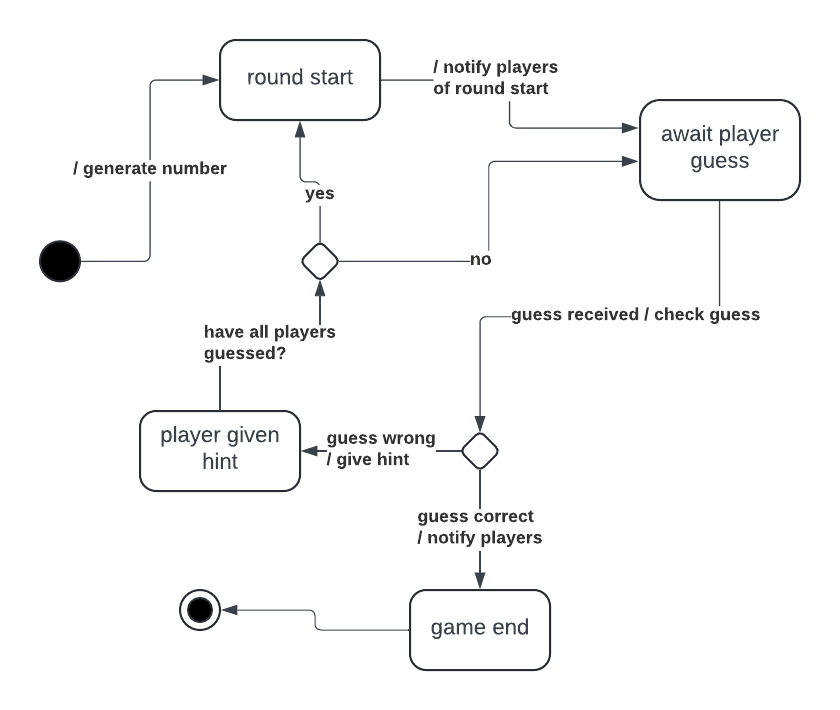
\includegraphics{oracleSD.png}
    \caption{state diagram of the oracle}
    \label{fig:oracleSD}
\end{figure}

\begin{figure}
    \centering
    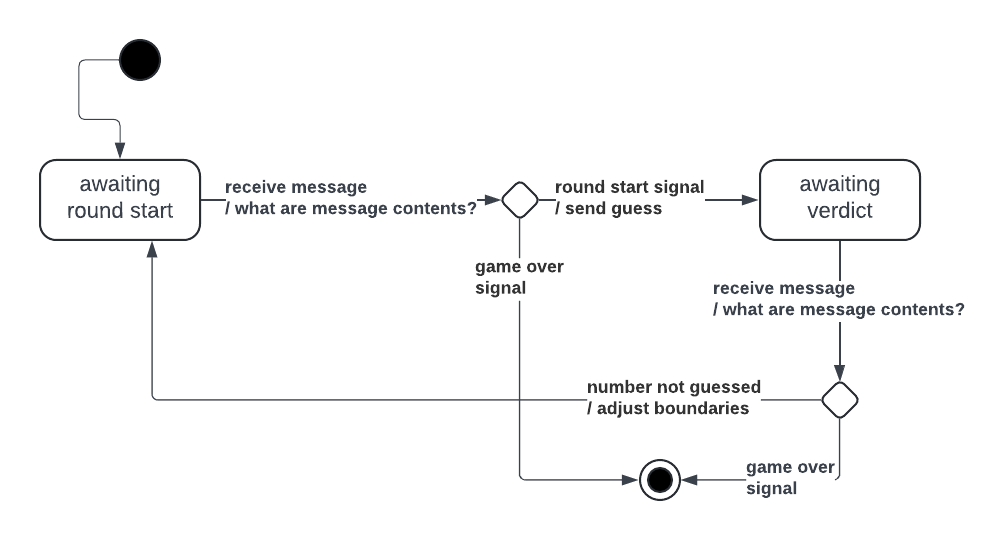
\includegraphics{playerSD.png}
    \caption{state diagram of a player}
    \label{fig:playerSD}
\end{figure}

\section{Communication organization}
Two choices where considered for channel organization:
\begin{itemize}
    \item Single channel for all communications
    \item A channel for every entity involved (one for the oracle and one for each player)
\end{itemize}

\newpage

Although using multiple channels involves a bigger overhead and reasource consumption, this approach was chosen for ease of use and to limit contention and
 the bottleneck risk of the single channel option.

The channels are treated as one way communication channels, where the entity the channel is associated to (oracle or player) is listening on the channel for messages.
 This means that if an entity wishes to communicate to a given other entity it can send messages on that entity's associated channel.

Since the players do not need to communicate with each other they have no need to have access to other player's channels, improving incapsulation //TODO CONTROLLARE COSA DIRE PER BENE QUI
\chapter{Implementation}
The oracle and players threads are implemented as goroutines. The goroutines communicate via channels.

The main file creates the oracle and players go routines.

The oracle go routine function is defined in the oracle.go file. The players go routine function is defined in the player.go file.

As defined in the Design chapter all the go routines have a single channel accosiated with them and each go routine listens only on their channel for messages from
 other go routines. This means that there are N + 1 channels, where N is the number of players.

The go routine functions for the oracle and the players where both implemented with a switch-case controll structure, highlighting the states
 rappresented in \ref{fig:oracleSD} and \ref{fig:playerSD}

This implementation takes into account an edge case where the oracle notifies the players that the game is over while a player has still not sent it's guess
 for the current round. Since the player considered would start listening to the it's channel after sending the message, it could send a possible guess
 before acknowledging that the game is over. Although this does not violate the requirements, it should be acknowledged that the player's go routines
 could terminate after the oracle routine and after the actual end of the game.

\section{Communication protocol}
Given the simple abstraction of channels a communication protocol must by defined. All the channels transport string type messages.

The oracle channel receives messages in the form of:
\begin{lstlisting}
    "<playerNumber> : <guess>"
\end{lstlisting}
Where \verb|<playerNumber>| is a number associated to the player and \verb|<guess>| is the player attempt at guessing the secret number.

The player channels receive messages in three different forms:
\begin{lstlisting}
    "wrong : <hint>"
    "gameover : <playerStatus>"
    "roundStart"
\end{lstlisting}
Where \verb|<hint>| is the hint from the oracle and can assume the value of \verb|higher| or \verb|lower| 
 and \verb|<playerStatus>| communicates to the player if they are the winner or not and can assume the value of \verb|winner| or \verb|loser|.

\chapter{Usage}
The program can be run from the command line using the command:
\begin{lstlisting}
    $ go run main.go oracle.go player.go oracleStates.go playerStates.go
\end{lstlisting}
The user will then be prompted to input the number of players and the max value for the number to be guessed.

The program can also be given the input values through cli arguments:
\begin{lstlisting}
    $ go run main.go oracle.go player.go oracleStates.go playerStates.go <nPlayers> <maxValue>
\end{lstlisting}
Where \verb|<nPlayers>| is the number of players.

Where \verb|<maxValue>| is the max value for the number to be guessed.

The program can also be run using either methods by running the given bash script:
\begin{lstlisting}
    $ ./runGame
\end{lstlisting}
\begin{lstlisting}
    $ ./runGame <nPlayers> <maxValue>
\end{lstlisting}

\chapter{Conclusions}
The go routine and channel constructs of the go language give supply an easy to use architecture for message oriented concurrency. Aided by the efficent Implementation
 of the go language, these simple yet powerfull abstractions allow to easily define complex beheviours in an intuitive and readable manner.

\bibliographystyle{plain}
\bibliography{References}

\end{document}